\documentclass{beamer}
\usepackage{graphicx,tabularx}
\usepackage{amsmath}
\usepackage{multicol}

\graphicspath{ {./source/} }
\usepackage[utf8]{inputenc}

\title{Comparison of network complexity measures}
\author{Yipei Zhao}
\institute{Aston University}
\date{\today}

\begin{document}
    \frame{\titlepage}
    \begin{frame}{Network Science}
        \centering
        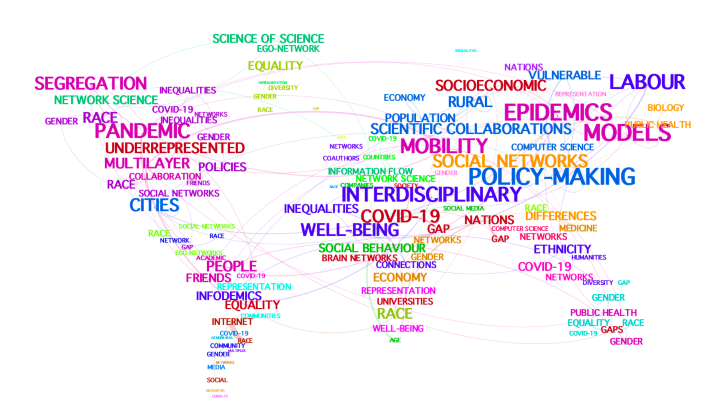
\includegraphics[width=\textwidth]{v1.png}
    \end{frame}


    \begin{frame}{Complexity measures}
        \begin{itemize}
            \item Different subgraph measures
            \begin{itemize}
                \item $C_{1e.st}$
                \item $C_{1e,spec}$
                \item $C_{2e,spec}$
            \end{itemize}
            \item Product measures
            \begin{itemize}
                \item $MA_g$
                \item $MA_{RI}$
                \item $Cr$
                \item $Ce$
            \end{itemize}
            \item Entropy measure
            \begin{itemize}
                \item $OdC$
            \end{itemize}
        \end{itemize}
    \end{frame}


    \begin{frame}{$MA_{RI}$}
        A product measure that is based on the idea of $MA_g$.
        \begin{itemize}
            \item Redundancy of a graph: $R=\frac{1}{m}\sum_{i,j>i}ln(d_id_j)$
            \item Mutual information of a graph: $I=\frac{1}{m}\sum_{i,j>i}ln(\frac{2m}{d_id_j})$
            \item An alternative way to state the mutual information: $I=ln(2m)-R$
            \item Highest redundancy: $R_{clique} = 2ln(n-1)$
            \item Lowest redundancy: $R_{path} = 2(\frac{n-2}{n-1})ln(2)$
            \item Highest mutual information: $I_{path} = ln(n-1)-(\frac{n-3}{n-1})ln2$
            \item Lowest mutual information: $I_{clique}=ln(\frac{n}{n-1})$
        \end{itemize}
        We can define the complexity to be $C = (R - R_{path})(I-I_{clique})$. 
    \end{frame}

    \begin{frame}{$MA_{RI}$ continue}
        To compare different complexity measures, they need to be normalised: $0<C<1$.\\
        The complexity measure can be rewritten as: $C=(R-R_{path})(ln(2m)-R-I_{clique})$.\\
        \vspace{5mm}
        \centering
        $C = -R^2+(ln(2m)-I_{clique}+R_{path})R+(-R_{path}ln(2m)+R_{path}I_{clique})$
    \\
        \vspace{5mm}
        $R_{max} = \frac{ln(2m)-I_{clique}+R_{path}}{2}$\\
        \vspace{5mm}
        $C_{max} = \frac{(ln(2m)-I_{clique}-R_{path})^2}{4}$\\
        \vspace{5mm}
        $MA_{RI} = \frac{4(R-R_{path})(I-I_{clique})}{(ln(2m)-I_{clique}-R_{path})^2}$
    \end{frame}

    \begin{frame}{Result}
        \centering
        \vspace{-15mm}
        \begin{figure}
            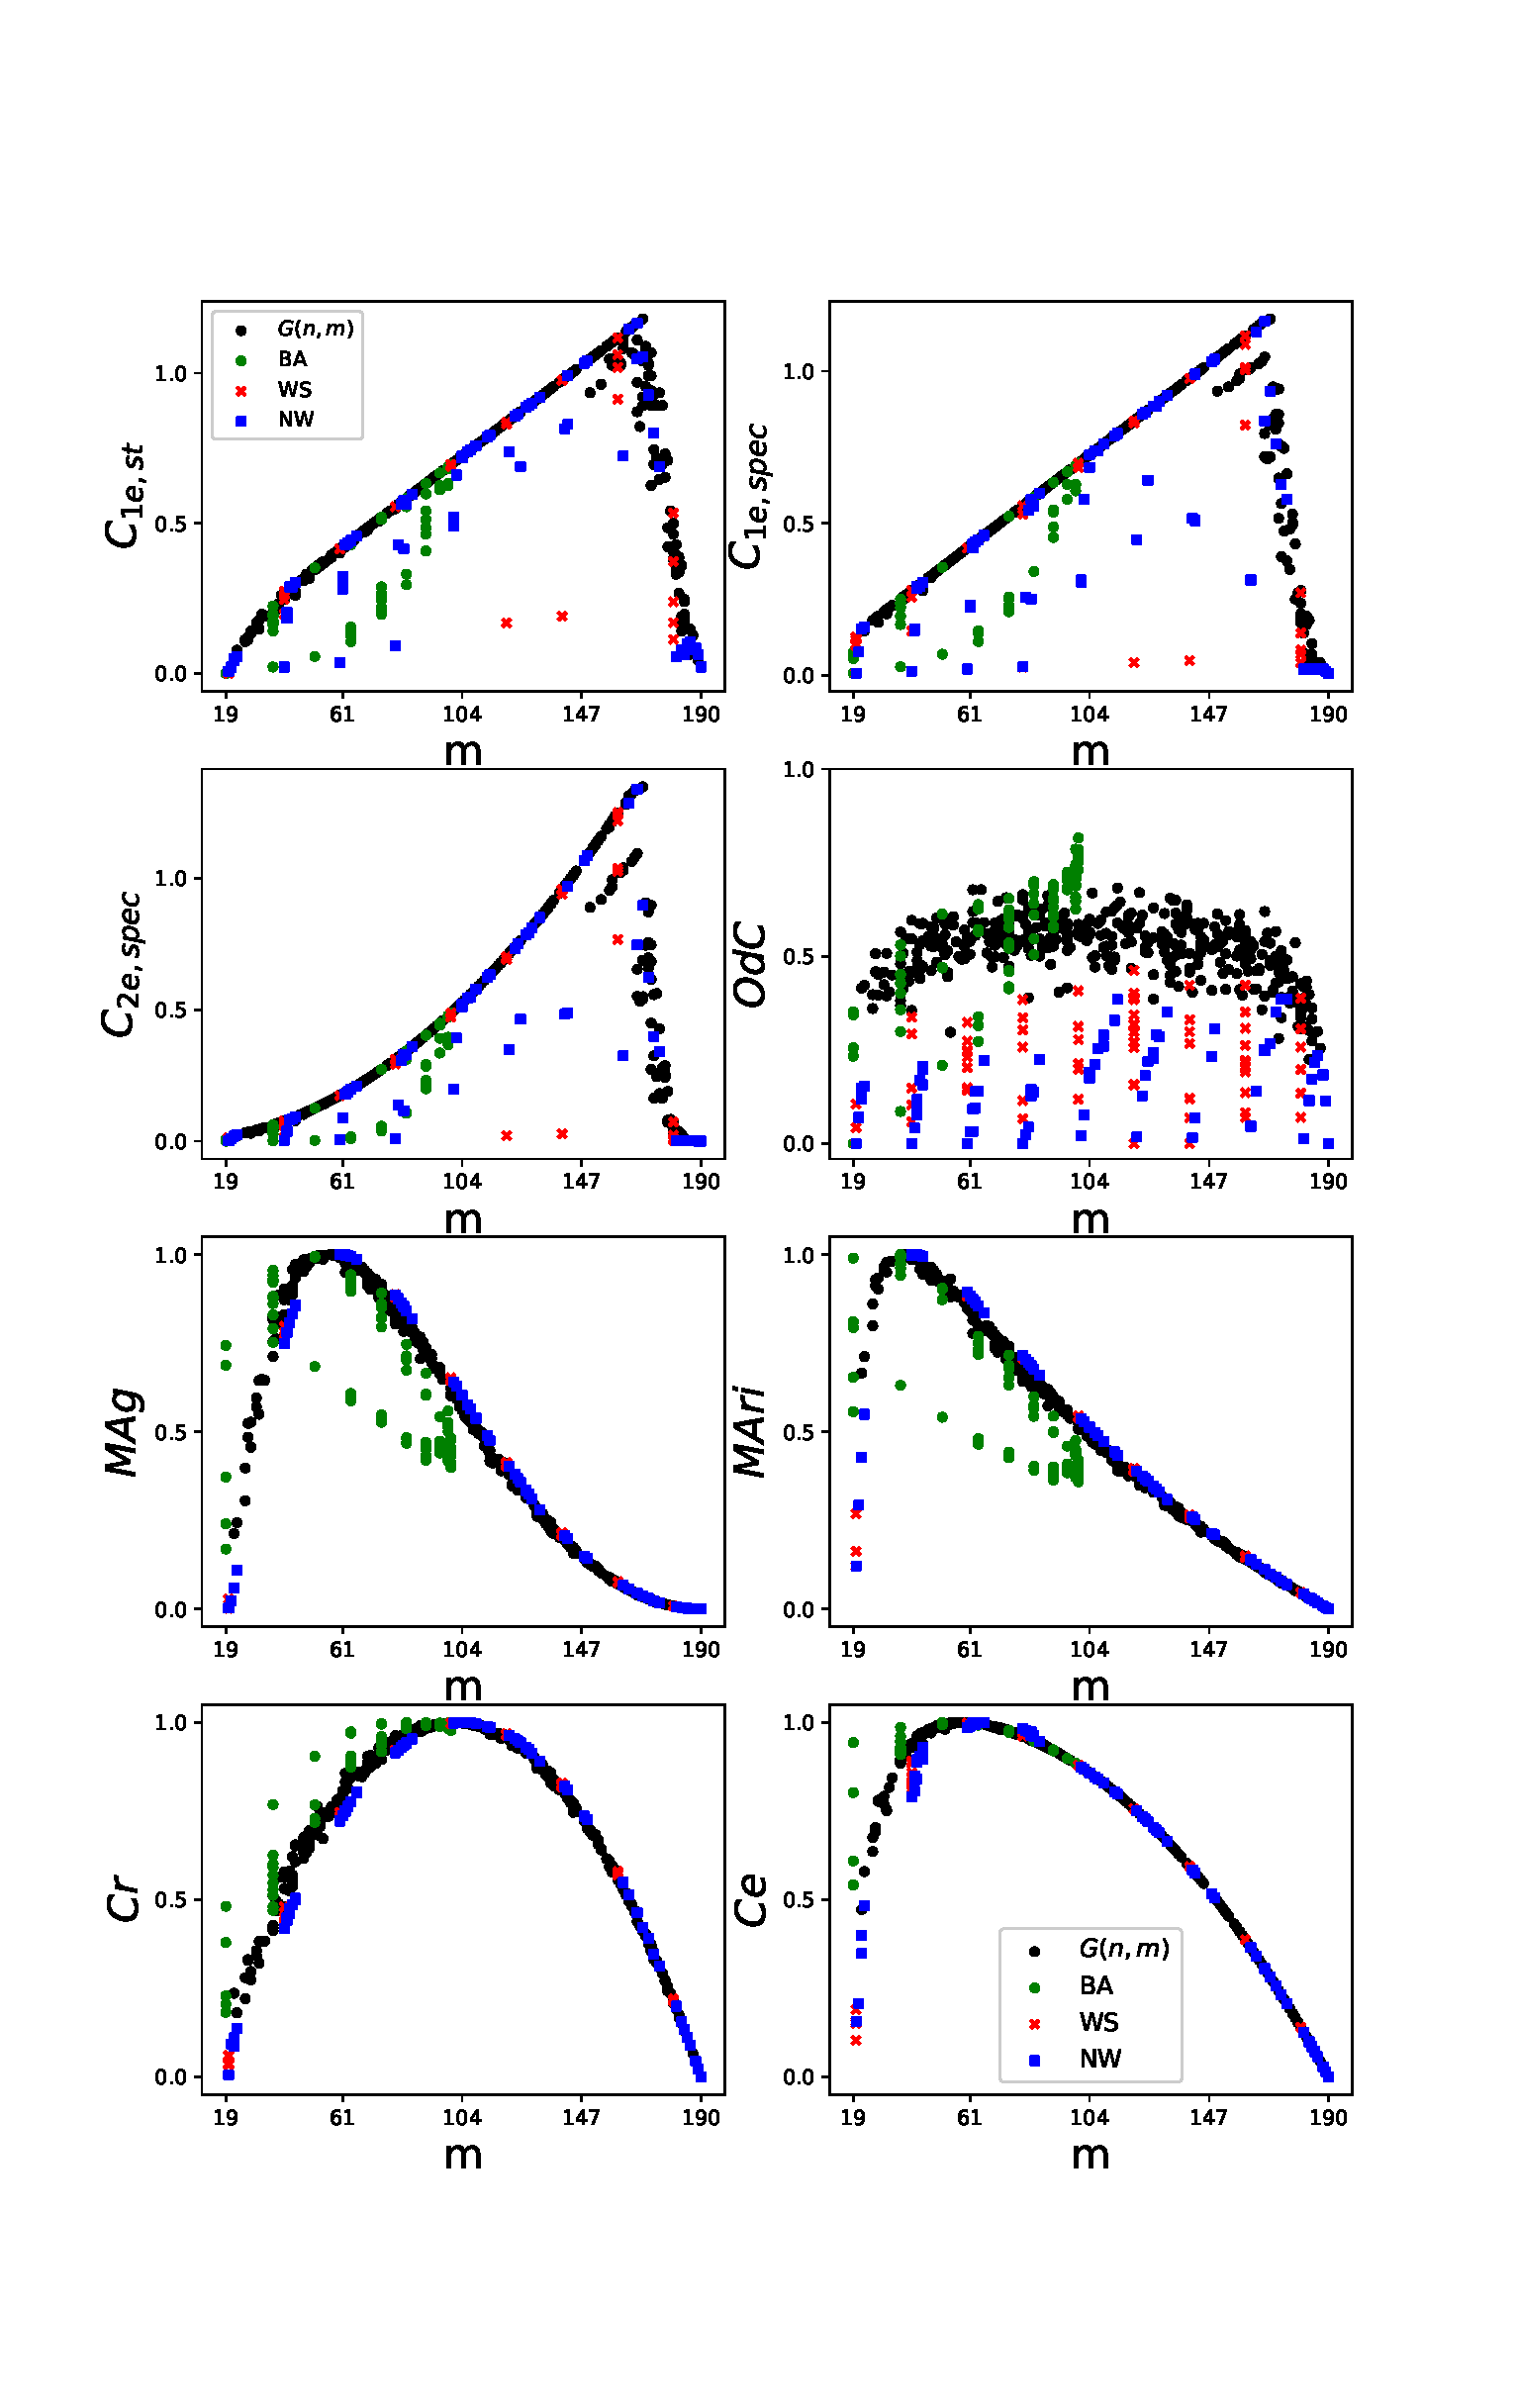
\includegraphics[width=\textwidth,height=\textheight,keepaspectratio]{complexities_sp.eps}
            \vspace{-8mm}
            \caption{Complexity of 500 $G(n,m)$ graphs, 100 BA graphs, 100 WS graphs and 100 NW graphs, with $n=20$.}
        \end{figure}
    \end{frame}

    \begin{frame}{Result continue}
        \vspace{-5mm}
            \begin{figure}
                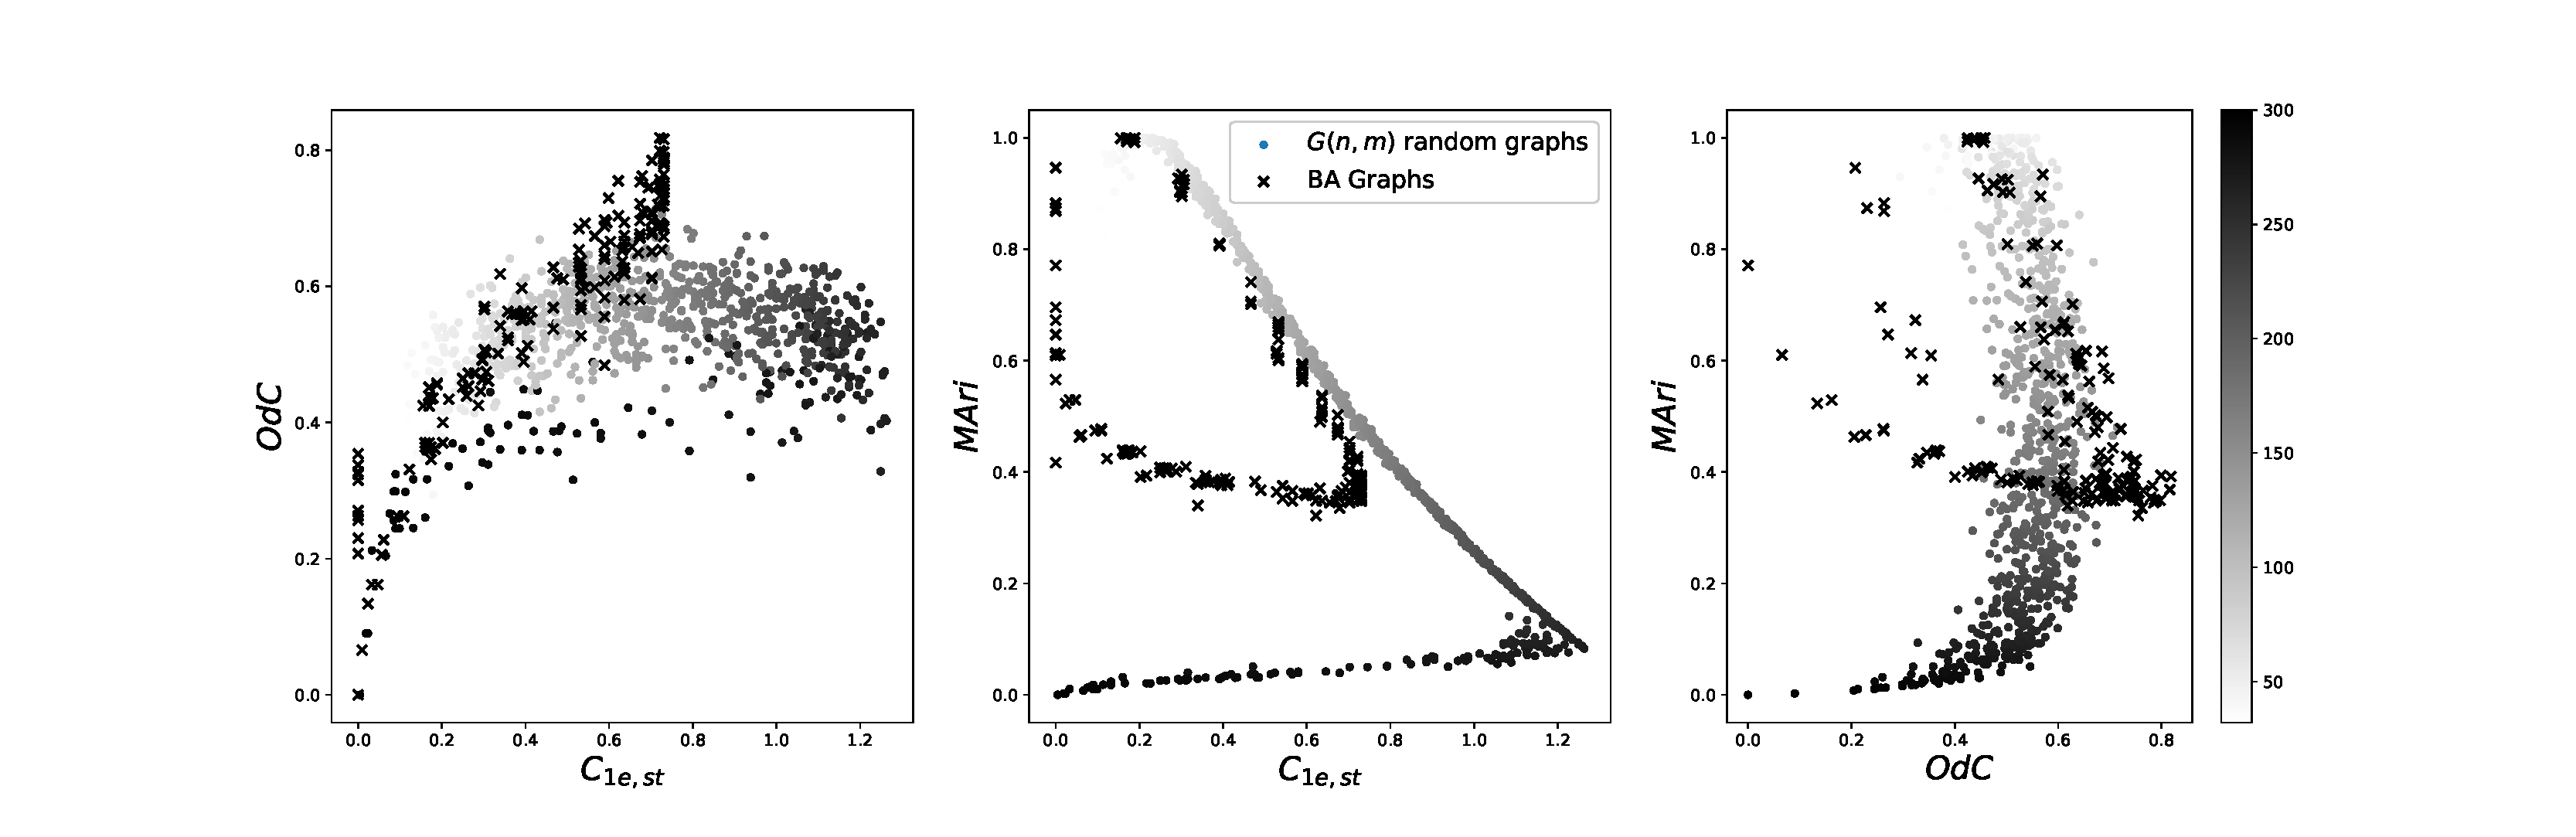
\includegraphics[width=\textwidth,height=0.5\textheight,keepaspectratio]{complexity_correlation.eps}
                \vspace{-10mm}
                \caption{Correlation between complexity measures, all graphs have 25 nodes and random number of edges. The darker the data point, the graph has more number of nodes.}
            \end{figure}
            \vspace{-15mm}
            \begin{figure}
                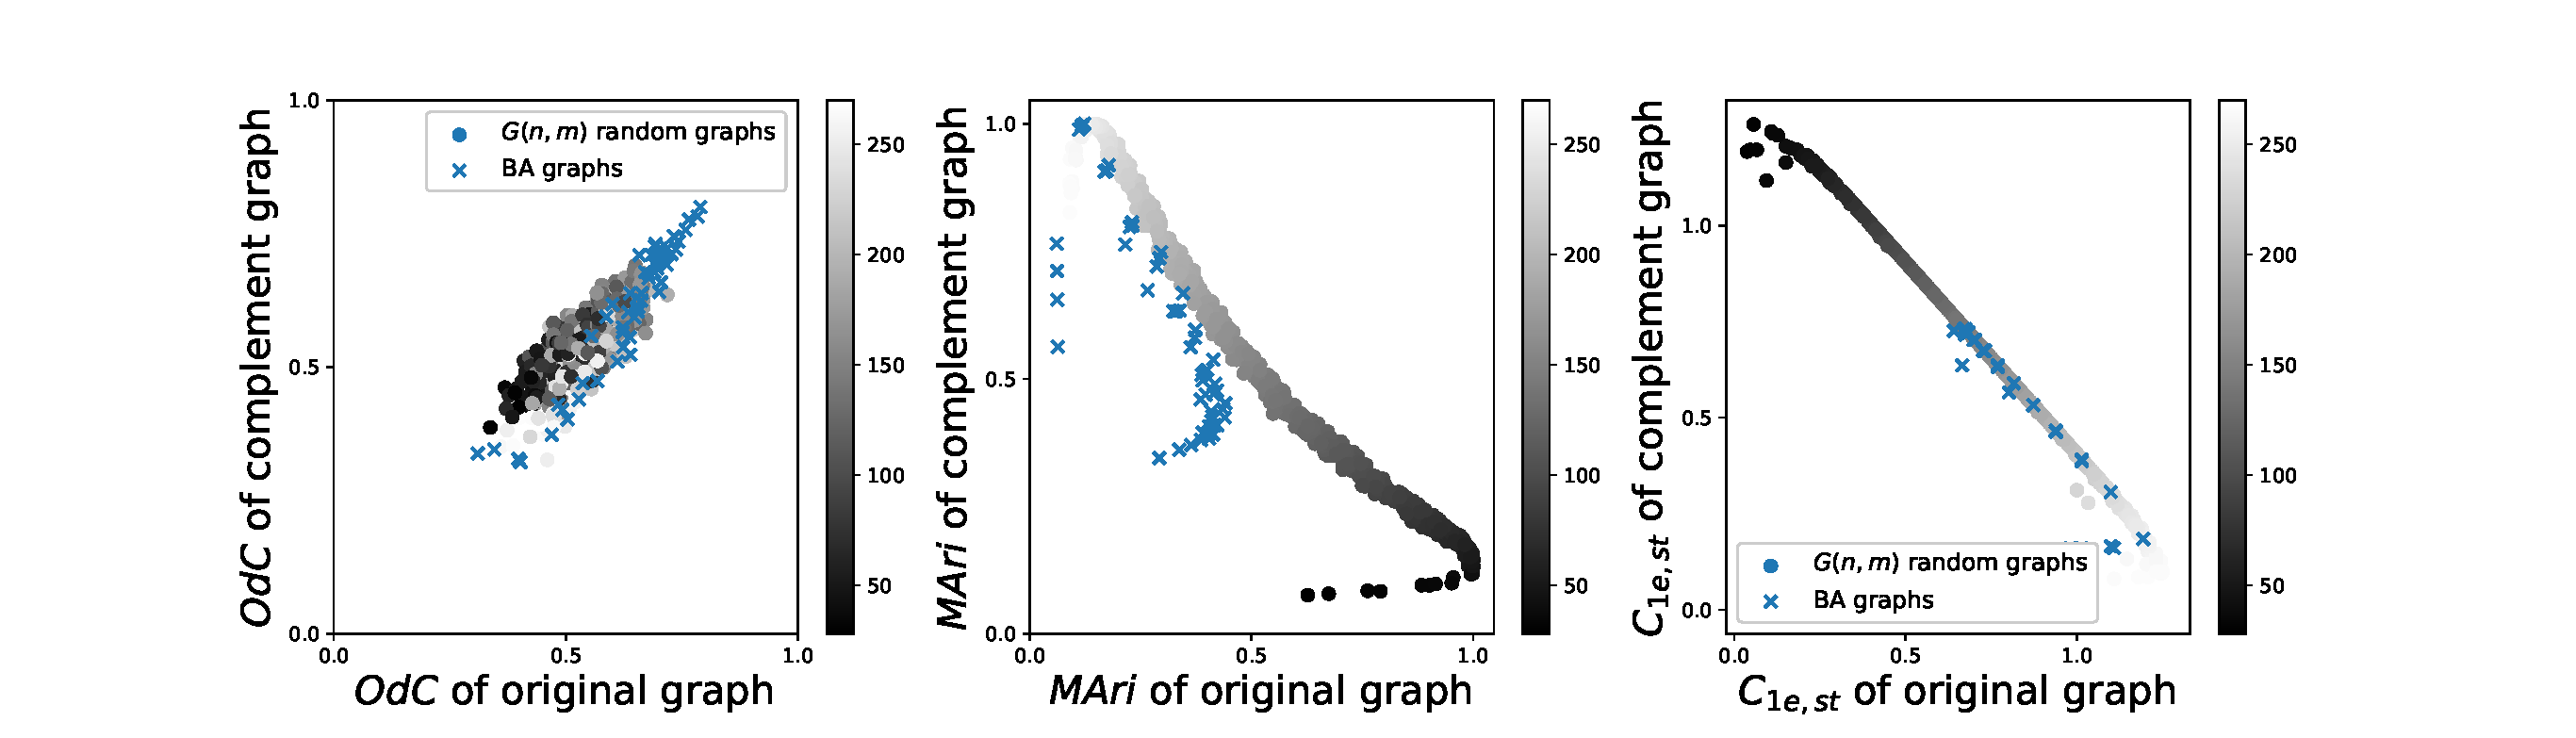
\includegraphics[width=\textwidth,height=0.5\textheight,keepaspectratio]{complement.eps}
                \caption{ Complexities of the original graphs and complement graphs with $n = 20$.}
            \end{figure}
    \end{frame}

    \begin{frame}{Result continue}
        \begin{figure}
            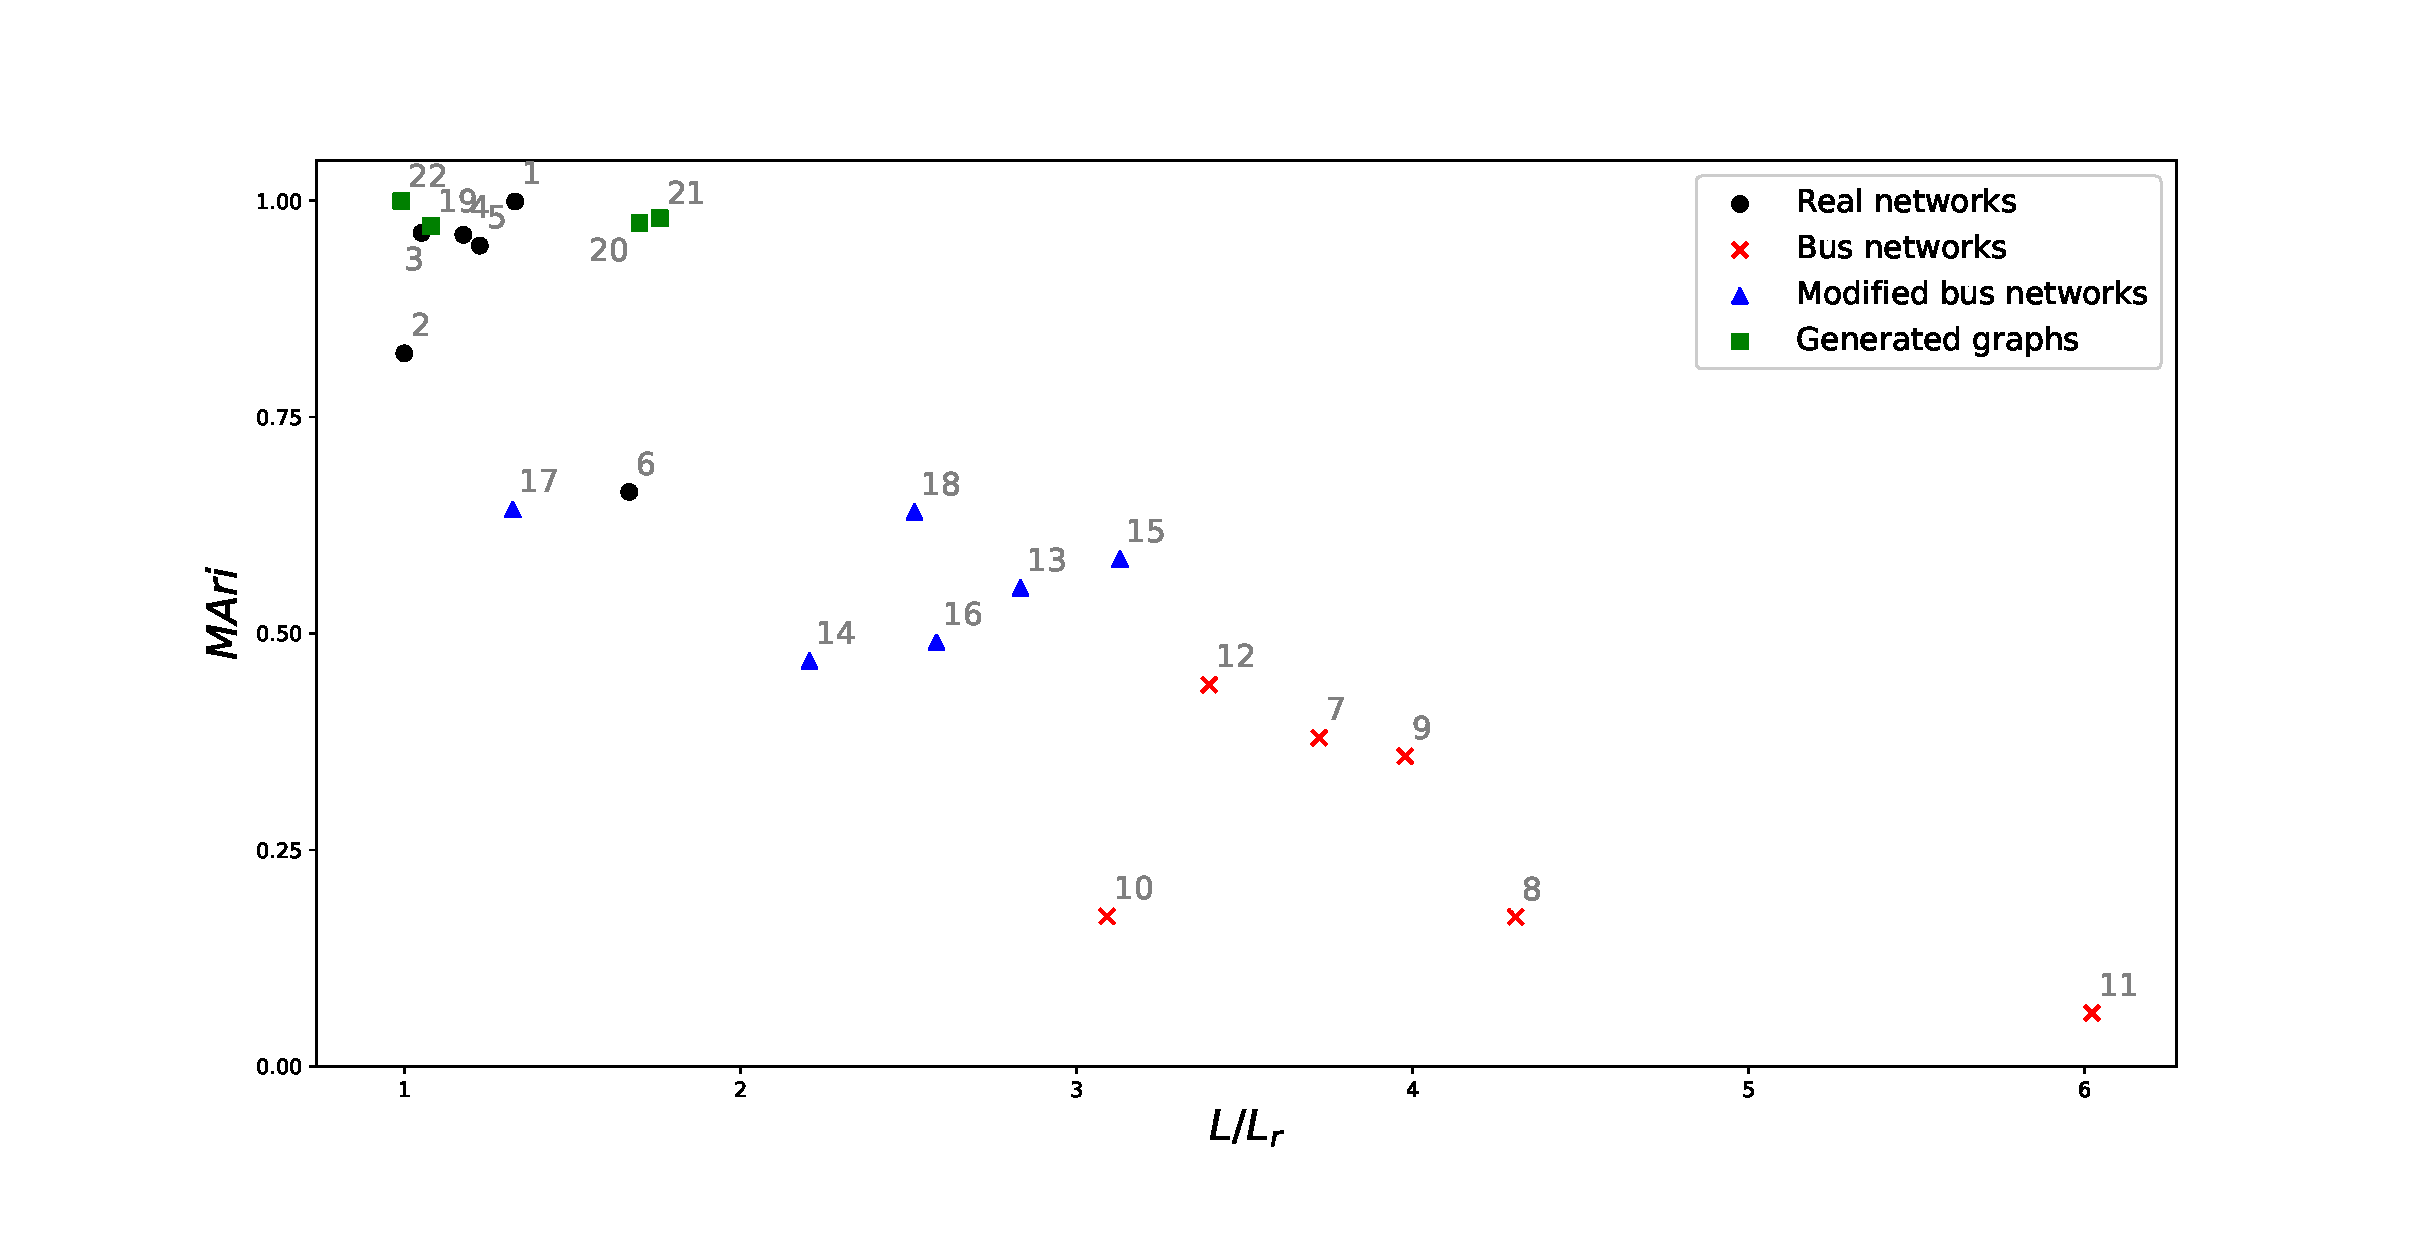
\includegraphics[width = \textwidth]{real_networks.eps}
            \caption{$MA_{RI}$ complexity of real networks, bus networks, modified bus networks and graphs generated by graph models.}
        \end{figure}
    \end{frame}

    \begin{frame}{Conclusion}
        \begin{itemize}
            \item Compared different complexity measures
            \item Introduced $MA_{RI}$
            \item Compared complexity measures on different types of graph
            \item Investigated the uniqueness of transportation networks
        \end{itemize}
    \end{frame}

    \begin{frame}{Reference}
        \begin{enumerate}
            \item {\url https://appliednetsci.springeropen.com/networked-inequality--studies-on-diversity-and-marginalization}
        \end{enumerate}        
    \end{frame}
\end{document}